\chapter{Confluencia}

En este capítulo estudiaremos el problema de determinar si un sistema
de reescritura es confluente. En la primera sección vamos a demostrar
que este problema es indecidible para el caso general. Sin embargo en
las secciones posteriores, estudiaremos que ocurre para un sistema
terminante. Para este caso el problema será decidible. Por último
veremos que podemos decir para los sistemas que no terminan.

\section{Estudio sobre el problema de decisión}
  
En esta sección veremos la indecibilidad para comprobar si un sistema
es confluente mediante el siguiente resultado,

\begin{teor}
  El problema de decidir si un sistema de reescritura finito $R$ es
  confluente, es indecidible.
\end{teor}

\begin{demo}
  El objetivo de esta demostración es reducir el problema de las
  palabras básicas para $E$ (que sabemos que es indecidible), a un
  sistema de reescritura de términos.

  Sea un conjunto de identidades $E$ tal que $\Var(l) = \Var(r)$ para
  todo $l \approx r \in E$. Sea $R := E \cup E^{-1}$, entonces al
  tener $\rightarrow_R = \leftrightarrow_E$ es confluente. Además $R$
  es un sistema de reescritura (por $\Var(l) = \Var(r)$).

  Dados dos términos básicos $s$ y $t$, y una constante $a$, vamos a
  probar que $R_{st} := R \cup \{ a \rightarrow s, a \rightarrow t \}$
  es confluente syss $s \approx_E t$.

  \begin{itemize}
  \item $(\Rightarrow)$ Si $R_{st}$ es confluente, entonces ni $s$, ni
    $t$ poseen una constante $a$, luego $s \downarrow_{R_{st}} t$. Esto
    significa que las reglas $a \rightarrow s, a \rightarrow t$ no
    pueden ser usadas. Por tanto $\rightarrow_R = \leftrightarrow_E$ y
    $s \approx_E t$.

  \item $(\Rightarrow)$ Vamos a probar que para términos $u, v$, si
    $u \rightarrow_{R_{st}} v$ entonces $v^t \xrightarrow{*}_R u^t$,
    donde $u^t$ denota el resultado de sustituir las constantes $a$ en
    $u$ por $t$.

    Supongamos que $u \rightarrow_{R{_st}} v$. Distinguimos que reglas
    se usan.
    \begin{itemize}
    \item Si usamos $u \rightarrow_R v$, reemplazamos $a$ por $t$ para
      conseguir $u^t \rightarrow_R v^t$ y por tanto
      $v^t \rightarrow_R u^t$ al ser $R$ simétrico.
    \item Si usamos $a \rightarrow s$, entonces $u|_p = a$ y
      $v = u[s]_p$ para alguna posición $p$. Como $s \approx_E t$
      entonces $s \xrightarrow{*}_R t$. Obtenemos
      $v \xrightarrow{*}_R u[t]_p$ que conlleva a
      $v^t \xrightarrow{*}_R (u[t]_p)^t$. Pero $(u[t]_p)^t =
      u^t[t^t]_p = u^t[t]_p = u^t$.
    \item Si usamos $a \rightarrow t$ en la posición $p$, entonces
      $v^t = (u[t]_p)^t = u^t \xrightarrow{*}_R u^t$.
    \end{itemize}
    Por tanto, si $u \xrightarrow{*}_{R_{st}} u_i$, para $i= 1,2$,
    entonces $u_i \xrightarrow{*}_{R_{st}} u_i^t \xrightarrow{*}_R u^t$
    y obtenemos $u_1 \downarrow_{R_{st}}$
  \end{itemize}
\end{demo}

\section{Pares críticos}

En esta sección estudiaremos la decibilidad para sistemas de
reescritura finitos que sean localmente confluentes.

La necesidad de los pares críticos surge de la importancia a la hora
de aplicar las reglas de un sistema de reescritura. Para entender
mejor este concepto, plantearemos el siguiente ejemplo. Sea $s$ un
término, $R := \{ l_1 \rightarrow r_1, l_2 \rightarrow r_2 \}$ donde
$l_1, l_2$ son subtérminos de $s$. Según apliquemos la primera regla o
la segunda, obtendremos un nuevo término $t$.

\begin{figure}[h]
  \centering
  \begin{tikzpicture}[->,>=stealth',level/.style={sibling distance =
      5cm/#1, level distance = 1.5cm}]

\node{$s$}
    child {
      node[align=center]{$t_1$}
        edge from parent node[above left] {$l_1 \rightarrow r_1$}}
    child {
      node{$t_2$}
      edge from parent node[above right] {$l_2 \rightarrow r_2$}
    };
\end{tikzpicture}
\end{figure}

Sea $p_i$ las posiciones y $\sigma_i$ las sustituciones tal que
$s|_{p_i} = \sigma_i l_i$ y $t_i = s[\sigma_i r_i ]_{p_i}, i
=1,2$. Tenemos que estudiar como de relacionados están $p_1$ y $p_2$.

\begin{itemize}

\item \textbf{Caso 1}, $p_1$ y $p_2$ están en árboles separados. En este caso,
  se da la convergencia local. Por ejemplo, supongamos que partimos de
  la figura \ref{fig:caso1a}.

  \begin{figure}[h]
    \centering
    \begin{tikzpicture}
\draw (0,0) node[anchor=north]{}
  -- (10,0) node[anchor=north]{}
  -- (5,5) node[below]{}
  -- cycle
   (2,0) node[anchor=north]{}
  -- (4,0) node[anchor=north]{}
  -- (3,1) node[below]{}
  -- cycle
  
     (8,0) node[anchor=north]{}
  -- (6,0) node[anchor=north]{}
  -- (7,1) node[below]{}
  -- cycle
  ;
\node[below] at (3,0.8) {\LARGE $\sigma_1 l_1$};
\node[below] at (7,0.8) {\LARGE $\sigma_2 l_2$};
\node[below] at (5,4.7) {\huge $s$};
\end{tikzpicture}
\caption{Término del caso 1 sin aplicar ninguna regla}
\label{fig:caso1a}
\end{figure}

Si aplicamos $l_1 \rightarrow r_1$ o $l_2 \rightarrow r_2$ obtenemos
las figuras \ref{fig:caso1b} y \ref{fig:caso1c} respectivamente.

\begin{figure}[h]
    \centering
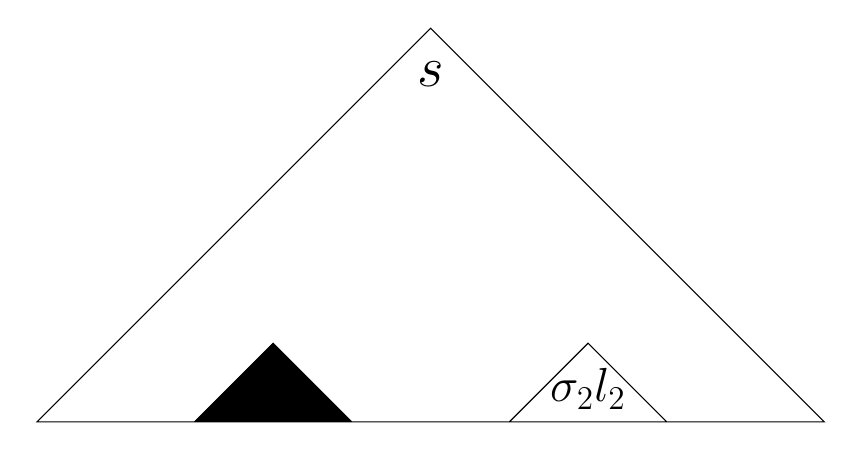
\begin{tikzpicture}
\draw (0,0) node[anchor=north]{}
  -- (10,0) node[anchor=north]{}
  -- (5,5) node[below]{}
  -- cycle
   (2,0) node[anchor=north]{}
  -- (4,0) node[anchor=north]{}
  -- (3,1) node[below]{}
  -- cycle
  
     (8,0) node[anchor=north]{}
  -- (6,0) node[anchor=north]{}
  -- (7,1) node[below]{}
  -- cycle
  ;
\node[below] at (3,0.8) {\LARGE $\sigma_1 l_1$};
\node[below] at (7,0.8) {\LARGE $\sigma_2 l_2$};
\node[below] at (5,4.7) {\huge $s$};

\node(a) at (2,0) {};
\node (b) at (4,0) {};
\node (c) at (3,1) {};
\fill (a.center) -- (b.center) -- (c.center);

\end{tikzpicture}
\caption{Término del caso 1 tras aplicar $l_1 \rightarrow r_1$}
\label{fig:caso1b}
\end{figure}

\begin{figure}[h]
\centering
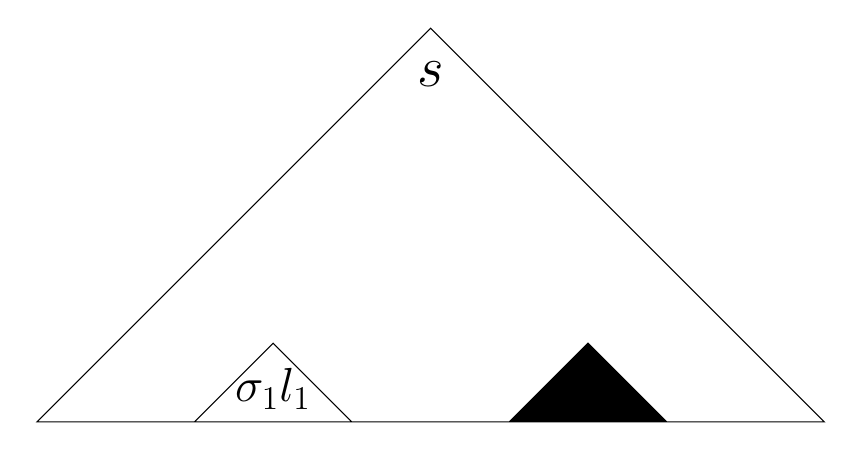
\begin{tikzpicture}
\draw (0,0) node[anchor=north]{}
  -- (10,0) node[anchor=north]{}
  -- (5,5) node[below]{}
  -- cycle
   (2,0) node[anchor=north]{}
  -- (4,0) node[anchor=north]{}
  -- (3,1) node[below]{}
  -- cycle
  
     (8,0) node[anchor=north]{}
  -- (6,0) node[anchor=north]{}
  -- (7,1) node[below]{}
  -- cycle
  ;
\node[below] at (3,0.8) {\LARGE $\sigma_1 l_1$};
\node[below] at (7,0.8) {\LARGE $\sigma_2 l_2$};
\node[below] at (5,4.7) {\huge $s$};

\node(a) at (8,0) {};
\node (b) at (6,0) {};
\node (c) at (7,1) {};
\fill (a.center) -- (b.center) -- (c.center);

\end{tikzpicture}
\caption{Término del caso 1 tras aplicar $l_2 \rightarrow r_2$}
\label{fig:caso1c}
\end{figure}

Y si usamos la regla que no se ha aplicado antes, para ambos términos
llegamos a la figura \ref{fig:caso1d}.

\begin{figure}[h]
\centering
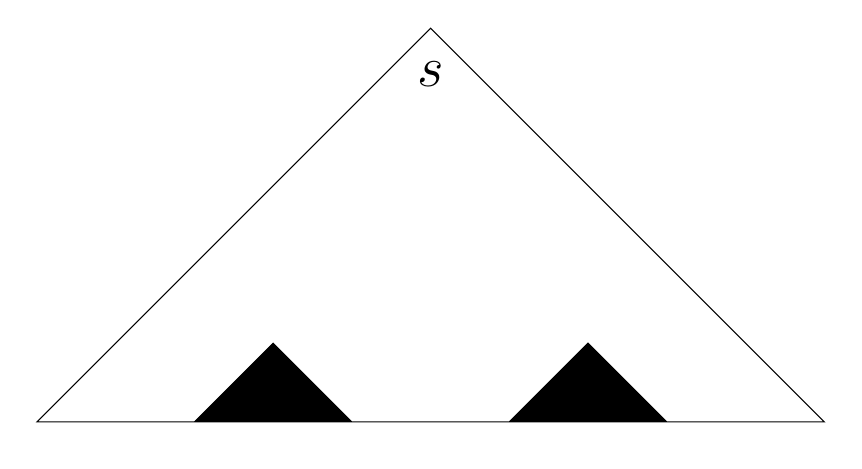
\begin{tikzpicture}
\draw (0,0) node[anchor=north]{}
  -- (10,0) node[anchor=north]{}
  -- (5,5) node[below]{}
  -- cycle
   (2,0) node[anchor=north]{}
  -- (4,0) node[anchor=north]{}
  -- (3,1) node[below]{}
  -- cycle
  
     (8,0) node[anchor=north]{}
  -- (6,0) node[anchor=north]{}
  -- (7,1) node[below]{}
  -- cycle
  ;
\node[below] at (3,0.8) {\LARGE $\sigma_1 l_1$};
\node[below] at (7,0.8) {\LARGE $\sigma_2 l_2$};
\node[below] at (5,4.7) {\huge $s$};

\node(a) at (8,0) {};
\node (b) at (6,0) {};
\node (c) at (7,1) {};
\node(a2) at (2,0) {};
\node (b2) at (4,0) {};
\node (c2) at (3,1) {};
\fill (a.center) -- (b.center) -- (c.center);
\fill (a2.center) -- (b2.center) -- (c2.center);

\end{tikzpicture}
\caption{Término en el caso 1, donde no se produce solapamiento}
\label{fig:caso1d}
\end{figure}

  
\item \textbf{Caso 2}. Si $p_1$ es un prefijo de $p_2$, tal y como se
  muestra en la figura \ref{fig:caso2}

\begin{figure}[h]
  \centering
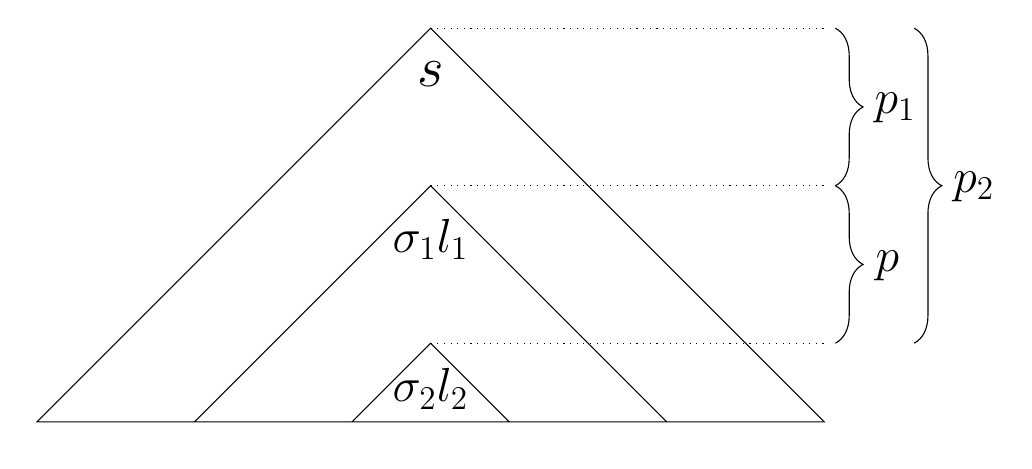
\begin{tikzpicture}
\draw[dotted](5,3)--(10,3);
\draw[dotted](5,5)--(10,5);
\draw[dotted](5,1)--(10,1);

\draw [decorate,decoration={brace,amplitude=10pt,mirror,raise=4pt},yshift=0pt]
(10,1) -- (10,3) node [black,midway,xshift=0.8cm] {};

\draw [decorate,decoration={brace,amplitude=10pt,mirror,raise=4pt},yshift=0pt]
(10,3) -- (10,5) node [black,midway,xshift=0.8cm] {};

\draw [decorate,decoration={brace,amplitude=10pt,mirror,raise=4pt},yshift=0pt]
(11,1) -- (11,5) node [black,midway,xshift=0.8cm] {};


\draw (0,0) node[anchor=north]{}
  -- (10,0) node[anchor=north]{}
  -- (5,5) node[below]{}
  -- cycle
   (2,0) node[anchor=north]{}
  -- (8,0) node[anchor=north]{}
  -- (5,3) node[below]{}
  -- cycle
  
     (4,0) node[anchor=north]{}
  -- (6,0) node[anchor=north]{}
  -- (5,1) node[below]{}
  -- cycle
  ;

\node[below] at (5,4.7) {\huge $s$};
\node[below] at (5,2.7) {\LARGE $\sigma_1 l_1$};
\node[below] at (5,0.8) {\LARGE $\sigma_2 l_2$};
\node[below] at (10.9,4.3) {\LARGE $p_1$};
\node[below] at (10.8,2.3) {\LARGE $p$};
\node[below] at (11.9,3.3) {\LARGE $p_2$};
\end{tikzpicture}
\caption{Situación del caso 2.}
\label{fig:caso2}
\end{figure}


A partir del dibujo, podemos distinguir dos casos según como de
separadas estén los términos $\sigma_1 l_1$ y $\sigma_2 l_2$.

  \begin{itemize}

  \item \textbf{Caso 2.1}. La reducción $\sigma_2 l_2$ no se solapa
    con $l_1$ pero está contenido en $\sigma_1$ (figura
    \ref{caso2a}). A esta situación la llamaremos solapamiento no
    crítico, pues en esta situación ocurre una confluencia local.

\begin{figure}[h]
  \centering
\usetikzlibrary{decorations.pathmorphing}
  \begin{tikzpicture}
\draw[dotted](5,3)--(10,3);
\draw[dotted](5,5)--(10,5);
\draw[dotted](5,2)--(10,2);

\draw(3,3)--(7,3);

\draw [decorate,decoration={brace,amplitude=10pt,mirror,raise=4pt},yshift=0pt]
(10,2) -- (10,3) node [black,midway,xshift=0.8cm] {};

\draw [decorate,decoration={brace,amplitude=10pt,mirror,raise=4pt},yshift=0pt]
(10,3) -- (10,5) node [black,midway,xshift=0.8cm] {};

\draw [decorate,decoration={brace,amplitude=10pt,mirror,raise=4pt},yshift=0pt]
(11,2) -- (11,5) node [black,midway,xshift=0.8cm] {};

\draw (0,0) node[anchor=north]{}
  -- (10,0) node[anchor=north]{}
  -- (5,5) node[below]{}
  -- cycle
  
     (3,0) node[anchor=north]{}
  -- (7,0) node[anchor=north]{}
  -- (5,2) node[below]{}
  -- cycle
  ;
  
\node[below] at (5,4.3) {\huge $l_1$};
\node[below] at (5,2.8) {\LARGE $\sigma_1$};
\node[below] at (5,1.2) {\LARGE $\sigma_2 l_2$};
\node[below] at (10.9,4.3) {\LARGE $q_1$};
\node[below] at (10.9,2.8) {\LARGE $q_2$};
\node[below] at (11.9,3.3) {\LARGE $p$};
\end{tikzpicture}
\caption{Caso 2.1.}
\label{fig:caso2a}
\end{figure}
    
\item \textbf{Caso 2.2}. En este caso $l_1$ y $l_2$ se solapan (figura
  \ref{caso2b}). A este caso lo llamaremos solapamiento crítico, y es
  la peor situación que podemos tener.

 \begin{figure}
      \centering
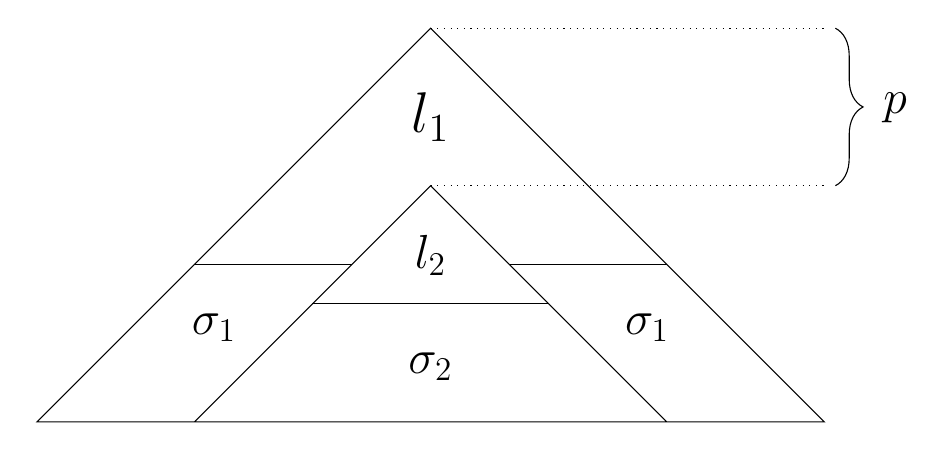
\begin{tikzpicture}


\draw[dotted](5,3)--(10,3);
\draw[dotted](5,5)--(10,5);


\draw(4,2)--(2,2);
\draw(6,2)--(8,2);
\draw(3.5,1.5)--(6.5,1.5);


\draw [decorate,decoration={brace,amplitude=10pt,mirror,raise=4pt},yshift=0pt]
(10,3) -- (10,5) node [black,midway,xshift=0.8cm] {};


\draw (0,0) node[anchor=north]{}
  -- (10,0) node[anchor=north]{}
  -- (5,5) node[below]{}
  -- cycle
  
     (2,0) node[anchor=north]{}
  -- (8,0) node[anchor=north]{}
  -- (5,3) node[below]{}
  -- cycle
  ;
  
\node[below] at (5,4.3) {\huge $l_1$};
\node[below] at (5,2.5) {\LARGE $l_2$};
\node[below] at (5,1) {\LARGE $\sigma_2$};
\node[below] at (2.25,1.5) {\LARGE $\sigma_1$};
\node[below] at (7.75,1.5) {\LARGE $\sigma_1$};
\node[below] at (10.9,4.3) {\LARGE $p$};

\end{tikzpicture}

\caption{Caso 2.2.}
\label{caso2b}
    \end{figure}    
  \end{itemize}


\end{itemize}


\begin{defi}
  Sea $l_i \rightarrow r_i$, $i = 1,2$ dos reglas cuyas variables han
  sido renombradas tal que
  $\Var(l_1,r_1) \cap \Var(l_2,r_2) = \emptyset$. Sea
  $p \in \Pos(l_1)$ tal que $l_1|_p$ no es una variable, y $\theta$ un
  umg de $l_1|_p =^? l_2$. Esto determinará el par crítico $\langle
  \theta r_1, (\theta l_1) [\theta r_2 ]_p \rangle$.
  % DIBUJO DEL ARBOL
  Si dos reglas dan lugar a un par crítico, diremos que se solapan.
\end{defi}

% EJEMPLO

A continuación enunciamos el Teorema de los Pares Críticos. Este
resultado así como la idea de la demostración, también se usará en la
siguiente sección.
\begin{teor}
  Un sistema de reescritura es localmente confluente syss todos sus
  pares críticos se vuelven a unir.
\end{teor}

\begin{demo}
  ($\Leftarrow$) Sabemos que si $s \rightarrow_R t$ para $i = 1,2$,
  entonces es localmente confluente, ó $t_i = s[u_i]_p$, donde
  $\langle u_1, u_2 \rangle$ proviene de algún par crítico
  $\langle v_1, v_2 \rangle$, es decir $u_1 = \delta v_i$. Entonces
  $\xrightarrow{*}t$ para algún término, y por tanto
  $u_i \xrightarrow \delta t$ es también cierto. Esto implica
  $t_i \xrightarrow s[\delta t]_p$ para $i = 1,2$.

  ($\Rightarrow$) Como el sistema de reescritura es localmente
  confluente, esto significa que cuando lleguemos a un par crítico
  este volverá a converger a un término. Luego todos sus pares
  críticos se vuelven a unir.
\end{demo}

Algunas propiedades directas de este teorema,

\begin{coro}\label{parcritcor}
  Un sistema de términos terminante es confluente syss todos sus pares
  críticos se vuelven a unir
\end{coro}

Pero si además pedimos que sea un sistema finito, obtenemos el
siguiente resultado.

\begin{coro}
  La confluencia de un sistema de reescritura finito y terminante es
  decidible.
\end{coro}

\begin{demo}
  El algoritmo que seguiremos será el siguiente:

  Para cada par de reglas $l_1 \rightarrow r_1$ y
  $l_2 \rightarrow r_2$, y para cada $p \in \Pos(l_1)$, tal que
  $l_1|_p$ no es una variable, se genera un par crítico unificando las
  variables disjuntas de $l_1|_p$ y $l_2$.

  Para cada uno de esos pares críticos $\langle u_1, u_2 \rangle$
  reducimos $u_i$ a su forma normal $\tilde{u}_i$. Decimos que el
  sistema de reescritura es confluente syss
  $\tilde{u}_1 = \tilde{u}_2$ para todos sus pares críticos.

  Si se verifica $\tilde{u}_1 = \tilde{u}_2$, entonces por el
  corolario \ref{parcritcor}, el sistema es confluente.

  Si se da el caso de que existe algún par crítico no
  $\tilde{u}_1 \not = \tilde{u}_2$, entonces se da la situación
  $\tilde{u}_1 \xleftarrow{*} u_1 \leftarrow u \rightarrow u_2
  \xrightarrow{*} \tilde{u_2}$, que demostraría que no es confluente.
\end{demo}

\section{Implementación de los pares críticos}

Se implementarán una función para calcular los pares críticos. Antes
de poder definirla, se necesitarán varias funciones auxiliares. El
código se puede encontrar en el fichero \texttt{ParesCriticos.hs}.

Vamos a necesitar la librería de términos.
\begin{codigo}
import Terminos
\end{codigo}

\begin{itemize}
\item \texttt{(indiceMaximo t)} \index{\texttt{indiceMaximo}}es el mayor índice que aparece en
  \texttt{t}. Por ejemplo,
\begin{sesion}
>>> indiceMaximo (V ("x",3))
3
>> indiceMaximo (T "w" [V("x",4), V("z", 200), V("y", 1)])
200
\end{sesion}

Su código es,

\begin{codigo}
indiceMaximo :: Termino -> Indice
indiceMaximo (V (_,i)) = i
indiceMaximo (T _ ts) = maximum (map indiceMaximo ts)
\end{codigo}

\item \texttt{(renombraTermino n t)}\index{\texttt{renombraTermino}}
  es el termino resultante tras sumar a todos los índices de
  \texttt{t} el entero \texttt{n}. Por ejemplo,
\begin{sesion}
>>> renombraTermino 5 (V ("x",3)) 
V ("x",8)
>>> renombraTermino 3 (T "w" [V("x",4), V("z", 200), V("y", 1)])
T "w" [V ("x",7),V ("z",203),V ("y",4)]
\end{sesion}

Su código es,

\begin{codigo}
renombraTermino :: Int -> Termino -> Termino
renombraTermino n (V (x,i)) = V(x,i+n)
renombraTermino n (T f ts) = T f (map (renombraTermino n) ts)
\end{codigo}

\item \texttt{(parCritico c (l1,r1) (l2,r2)} \index{\texttt{parCritico}} calcula el par crítico de la
  regla $\texttt{l1} \rightarrow \texttt{r1}$ y
  $\texttt{l2} \rightarrow \texttt{r2}$. Por ejemplo,
\begin{sesion}
>>> let c a = a
>>> parCritico c (V ("x",1), T "f" [V ("y",1)])
                 (V ("x",2),T "g" [V("y",2)])
[(T "f" [V ("y",1)],T "g" [V ("y",2)])]
>>> parCritico c (T "f" [V ("x",1)],T "f" [V ("y",1)])
               (V ("x",1), T "g" [V("y",2)])
[]
\end{sesion}

Su código es,

\begin{codigo}
parCritico :: (Termino -> Termino) -> (Termino, Termino)
           -> (Termino, Termino) -> [(Termino, Termino)]
parCritico c (l1, r1) (l2, r2)
    | sigma1 == Left UNIFICACION = []
    | otherwise = [(sigma r1, sigma (c r2))]
    where sigma1 = unificacion l1 l2
          sigma = aplicaTerm (elimR(sigma1))
          elimR (Right a) = a
\end{codigo}

\item \texttt{(paresCriticos rlista (l,r))} \index{\texttt{paresCriticos}}calcula la lista de todos
  los pares críticos formados al unificar \texttt{rlista} hacia la
  izquierda con un subtérmino \texttt{l}, donde \texttt{l
    $\rightarrow$ r} es una regla. Por ejemplo,

\begin{sesion}
>>> paresCriticos [(V ("x",1), T "f" [V("y",1)])]
                  (V ("x",2), T "g" [V("y",2)])
[]
>>> paresCriticos [(T "f" [V ("x",1)], T "f" [V ("y",1)]),
                   (T "f"[V ("x",1)], T "g" [V ("x",2)]), 
                   (T "g" [V ("x",2)],  T "f" [V ("y",1)])] 
                   (V ("x",1), T "f" [V("y",1)])
[]
>>> paresCriticos [(T "f" [T "g" [V("x",1),V("y",1)],V("z",1)],
                    T "g" [V("x",1),V("z",1)]),
                   (T "g" [V("x",1),V("y",1)],V("x",1))]
                   (T "g" [V("x",1),V("y",1)],
                    T "g" [V("x",1),V("z",1)])
[(T "g" [V ("x",1),V ("z",3)],V ("x",1))]
\end{sesion}

Su código es,

\begin{codigo}
paresCriticos :: [(Termino, Termino)] -> (Termino, Termino)
                 -> [(Termino, Termino)]
paresCriticos rlista (l,r) =
    cps (\x -> x) (renombraTermino m l) (renombraTermino m r)
    where cps _ (V _) _ = []
          cps c ter@(T f ts) r1 = 
                concat(map (parCritico c (ter,r1)) rlista) ++
                 (pcint c f [] ts r1)(pcint c f [] ts r1)
          pcint _ _ _ [] _ = []
          pcint c f ts0 (t:ts1) r2 =
              (cps (\s -> c (T f (ts0++[s]++ts1))) t r2)
                          ++ (pcint c f (ts0++[t]) ts1 r2)
          m = maximum(map
               (\(l3,r3) ->
                maximum(indiceMaximo l3, indiceMaximo r3))
                 rlista) + 1
\end{codigo}

\item \texttt{(paresLista r)} \index{\texttt{paresLista}}es la lista de todos los pares críticos
  de \texttt{r}, incluyendo los triviales. Por ejemplo,

\begin{sesion}
>>> paresLista [(V ("x",1), T "f" [V("y",1)])]
[]
>>> paresLista [(T "f" [T "g" [V("x",1),V("y",1)],V("z",1)],
                 T "g"[V("x",1),V("z",1)]),
                (T "g" [V("x",1),V("y",1)],V("x",1))]
[(T "g" [V ("x",1),V ("z",1)], T "g" [V ("x",1),V ("z",1)]),
 (T "g" [V ("x",1),V ("z",3)], T "f" [V ("x",1),V ("z",3)]),
 (V ("x",1),V ("x",1))]
\end{sesion}

Su código es,

\begin{codigo}
paresLista :: [(Termino, Termino)] -> [(Termino, Termino)]
paresLista r1 = paresLista2 r1 r1
\end{codigo}

\item \texttt{(paresLista2 r1 r2)} \index{\texttt{paresLista2}}es la lista de todos los pares
  críticos al unificar los términos a la izquierda de \texttt{r1} con un
  subtérmino a la izquierda con \texttt{r2}. Por ejemplo,

\begin{sesion}
>>> paresLista2 [(V ("x",1), T "f" [V("y",1)])]
                [(V ("x",1), T "f"[V("y",1)])]
[]
>>> paresLista2 [(T "f" [T "g" [V("x",1),V("y",1)],V("z",1)],
                  T "g"[V("x",1),V("z",1)]),
                 (T "g" [V("x",1),V("y",1)],V("x",1))]
                [(V ("x",1), T "f" [V("y",1)])] 
[]
>>> paresLista2 [(V ("x",1), T "f" [V("y",1)])] 
                [(T "f" [T "g" [V("x",1),V("y",1)],V("z",1)],
                  T "g"[V("x",1),V("z",1)]),
                  (T "g" [V("x",1),V("y",1)],V("x",1))]
[(T "g" [V ("x",3),V ("z",3)],T "f" [V ("y",1)]),
 (T "g" [V ("x",3),V ("z",3)],
  T "f" [T "f" [V ("y",1)],V ("z",3)]),
 (V ("x",3),T "f" [V ("y",1)])]
\end{sesion}

Su código es,

\begin{codigo}
paresLista2 :: [(Termino, Termino)] -> [(Termino, Termino)]
               -> [(Termino, Termino)]
paresLista2 r1 r2 = concat(map(paresCriticos r1) r2)
\end{codigo}

\end{itemize}

\section{Ortogonalidad}

En la sección anterior hemos analizado una técnica para determinar la
confluencia para sistemas terminantes. En esta nos dedicaremos a
analizar el problema para sistemas no terminantes. Para ello la
estudiaremos desde otra perspectiva usando nuevamente los pares
críticos.

\begin{defi}
  Una regla de reescritura $l \rightarrow r$ es lineal por la
  izquierda (respectivamente lineal por la derecha) si ninguna
  variable ocurre dos veces en $l$ (respectivamente $r$). Si una regla
  es lineal por la izquierda y por la derecha diremos que es lineal. 
\end{defi}

Y ampliamos la definición para sistemas de reescritura.

\begin{defi}
  Un sistema de reescritura es lineal por la izquierda
  (respectivamente por la derecha) si todas sus reglas son lineales por
  la izquierda (respectivamente por la derecha)
\end{defi}

Por último, antes de dar el principal resultado de la sección,
definimos una restricción que nos servirá para demostrar la
confluencia fuerte.

\begin{defi}
  Los términos $s_1$ y $s_2$ es fuertemente unible respecto
  $\rightarrow$ si existen términos $t_1$ y $t_2$ tal que
  $s_1 \xrightarrow{=} t_1 \xleftarrow{*} s_2$ y $s_1 \xrightarrow{*}
  t_2 \xleftarrow{=} s_2$
\end{defi}

% AÑADIR DIBUJO DEL ESTILO:
%    /s1\ 
%  t1    t2
%    \s2/

El siguiente resultado se conoce como el lema de confluencia fuerte.

\begin{defi}
  Si $R$ es lineal y cada par crítico de $R$ es fuertemente unible,
  entonces $R$ es fuertemente confluente.
\end{defi}

\begin{demo}
  La prueba se hará reduciendo cada uno de los casos que estudiamos en
  la sección anterior.
  
  \begin{itemize}
    
  \item Caso 1. Es trivial.

  \item Caso 2.1. Se simplifica mediante la restricción de linealidad
    % DIBUJO

  \item Caso 2.2. Como todos los pares críticos son fuertemente
    unible, la instancia de un par crítico es fuertemente unible

  \end{itemize}

\end{demo}

Si un sistema es fuertemente confluente, en particular, también es
confluente. Por tanto acabamos de probar una condición suficiente para la
confluencia.

% EJEMPLO

\begin{defi}
  Un sistema de reescritura es ortogonal si es lineal por la izquierda
  y no tiene pares críticos
\end{defi}

Probar la confluencia para un sistema ortogonal posee el siguiente
problema; al no poseer linealidad por la derecha, en el caso 2.1 es
posible que se aplique mas de una vez la reducción $l_2 \rightarrow r_2$,
y por tanto, lo único que podemos deducir es la confluencia
local. Para evitar este problema, usaremos una relación de reescritura
que posea la propiedad del diamante, que recordemos que el
cumplimiento de esta propiedad implica la confluencia.

Volviendo al caso 2.1, para conseguir la propiedad del diamante
tenemos que arreglar el problema de aplicar repetidas veces la
reducción $l_2 \rightarrow r_2$. Para ello vamos a considerar
reducciones paralelas para los subárboles. Es decir, si tenemos la
figura \ref{fig:pararb1}, consideramos la reducción
$\rightrightarrows$ con la que obtenemos la situación \ref{fig:pararb2}.

\begin{figure}
\centering
\usetikzlibrary{decorations.pathreplacing}
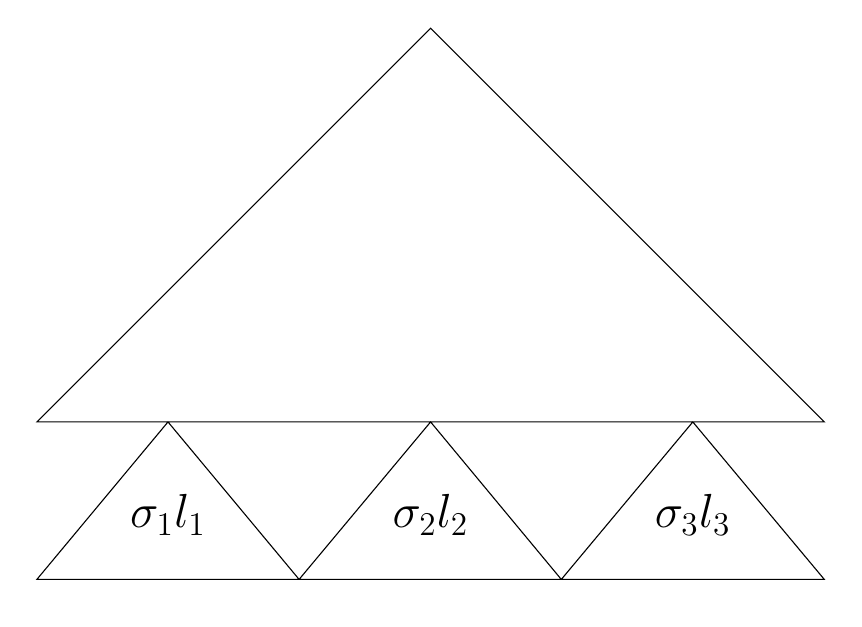
\begin{tikzpicture}

\draw (0,0) node[anchor=north]{}
  -- (10,0) node[anchor=north]{}
  -- (5,5) node[below]{}
  -- cycle
    
       (0,-2) node[anchor=north]{}
  -- (3.33,-2) node[anchor=north]{}
  -- (1.665,0) node[below]{}
  -- cycle
  
       (3.33,-2) node[anchor=north]{}
  -- (6.66,-2) node[anchor=north]{}
  -- (5,0) node[below]{}
  -- cycle
  
        (6.66,-2) node[anchor=north]{}
  -- (10,-2) node[anchor=north]{}
  -- (8.33,0) node[below]{}
  -- cycle
  ;
  

\node[below] at (1.665,-0.8) {\LARGE $\sigma_1 l_1$};
\node[below] at (5,-0.8) {\LARGE $\sigma_2 l_2$};
\node[below] at (8.33,-0.8) {\LARGE $\sigma_3 l_3$};

\end{tikzpicture}
\caption{}
\label{fig:pararb1}
\end{figure}

\begin{figure}
\centering
\usetikzlibrary{decorations.pathreplacing}
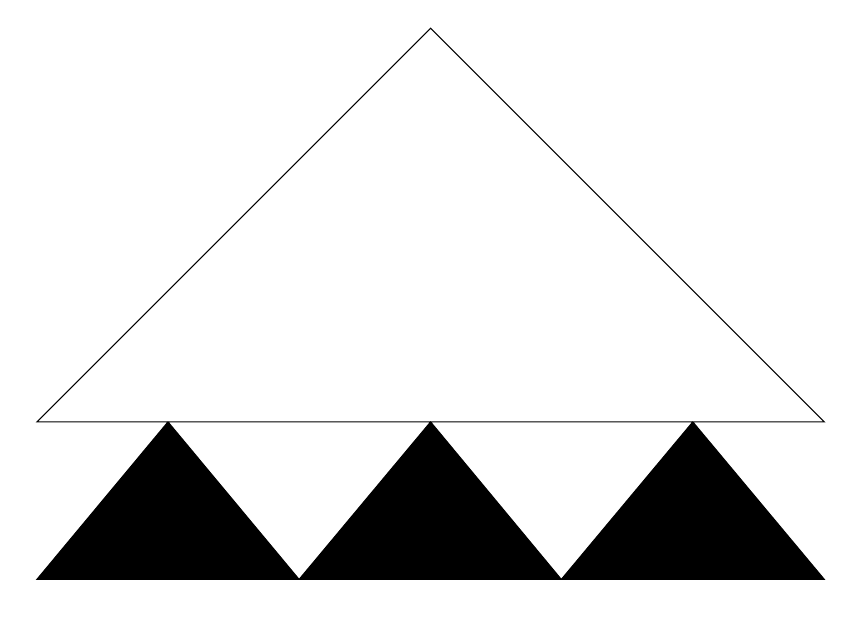
\begin{tikzpicture}

\draw (0,0) node[anchor=north]{}
  -- (10,0) node[anchor=north]{}
  -- (5,5) node[below]{}
  -- cycle
    
       (0,-2) node[anchor=north]{}
  -- (3.33,-2) node[anchor=north]{}
  -- (1.665,0) node[below]{}
  -- cycle
  
       (3.33,-2) node[anchor=north]{}
  -- (6.66,-2) node[anchor=north]{}
  -- (5,0) node[below]{}
  -- cycle
  
        (6.66,-2) node[anchor=north]{}
  -- (10,-2) node[anchor=north]{}
  -- (8.33,0) node[below]{}
  -- cycle
  ;

\node(a) at (0,-2) {};
\node (b) at (3.33,-2) {};
\node (c) at (1.665,0) {};
\node(a2) at (3.33,-2) {};
\node (b2) at (6.66,-2) {};
\node (c2) at (5,0) {};
\node(a3) at (6.66,-2) {};
\node (b3) at (10,-2) {};
\node (c3) at (8.33,0) {};
\fill (a.center) -- (b.center) -- (c.center);
\fill (a2.center) -- (b2.center) -- (c2.center);
\fill (a3.center) -- (b3.center) -- (c3.center);

\end{tikzpicture}

\caption{}
\label{fig:pararb2}
\end{figure}

\begin{defi}
  Diremos que un conjunto de posiciones es paralelo si $p||q$ para
  todo $p, q \in P$, donde $P$ es un subconjunto de todas las posibles
  posiciones paralelas.
\end{defi}

Dado un término $t_p$ para cada $p \in P$, definimos la notación,
\[ s[t_p]_{p\in P} : = s[t_{p_1}]_{p_1} \dots [t_{p_n}]_{p_n} \]

\begin{defi}
  Si para cada $p \in P$ tenemos la regla $l_p \rightarrow r_p in R$ y
  para cada sustitución $\sigma_p$ tal que $s|_p = \sigma_p l_p$
  llamaremos reducción paralela a
  $s \rightrightarrows^P_R s[\sigma_p r_p]_{p \in P}$
\end{defi}

A partir de esta definición, enunciamos el teorema de los sistemas
ortogonales

\begin{teor}
  Si $R$ es ortogonal entonces $\rightrightarrows_R$ tiene la
  propiedad del diamante
\end{teor}

\begin{demo}
  Sea $s \rightrightarrows^{P_i} t_i, i = 0,1$. Para esta prueba vamos
  a considerar una partición de $P_i = A_i \cup B_i \cup C$ donde
\begin{itemize}
\item $A_i := \{ p \in P_i | \not \exists q \in P_{1-i}, q \leq p \}$
\item $B_i := \{ p \in P_i | \exists q \in P_{1-i}, q < p \}$
\item $P_0 \cap P_1$
\end{itemize}

Analizamos que elementos hay en cada partición; $A_i$ contiene todas
las posiciones contraídas que estén por encima de
$s \rightrightarrows t_{1-i}$, $B_i$ contiene las que están por debajo
estrictamente de las contraídas en $s \rightrightarrows t_{1-i}$, y
$C$ un conjunto de posiciones contraídas en ambas reducciones.

Como no tenemos pares críticos, todos los $b_i$ son el resultado de
aplicar una regla de reducción hacia la derecha a $a_{1-i}$.

La reducción $t_{1-i} \rightrightarrows u$ tiene las mismas reglas que
las posiciones $B_i$. Lo mismo ocurre para $s \rightrightarrows
t_i$. Nuestro objetivo es llegar a que $t_{1-i} \rightrightarrows u$
también usa las posiciones de $A_i$, para llegar a formar el diamante.

Una reducción en la posición $a_i \in A_i$, no puede ser destruida por
una reducción de algún $b_{1-i} \in B_{1-i}$ porque $R$ es lineal por
la izquierda. Por tanto la reducción $t_{1-i} \rightrightarrows u$ usa
las mismas reglas en las posiciones $A_i$ en la reducción
$s \rightrightarrows t_i$ (que aplicadas en las posiciones de $B_i$).
\end{demo}

Y en particular, tenemos el siguiente corolario.

\begin{coro}
Todo sistema de reescritura ortogonal es confluente.
\end{coro}

%%% Local Variables:
%%% mode: latex
%%% TeX-master: "SRT_en_Haskell"
%%% End:
